%%%%%%%%%%%%%%%%%%%%%%%%%%%%%%%%%%%%%%%%%%%%%%%%%%%%%%%%%%%%%%%%%%%%
%% I, the copyright holder of this work, release this work into the
%% public domain. This applies worldwide. In some countries this may
%% not be legally possible; if so: I grant anyone the right to use
%% this work for any purpose, without any conditions, unless such
%% conditions are required by law.
%%%%%%%%%%%%%%%%%%%%%%%%%%%%%%%%%%%%%%%%%%%%%%%%%%%%%%%%%%%%%%%%%%%%

\documentclass[
  digital, %% This option enables the default options for the
           %% digital version of a document. Replace with `printed`
           %% to enable the default options for the printed version
           %% of a document.
  table,   %% Causes the coloring of tables. Replace with `notable`
           %% to restore plain tables.
  lof,     %% Prints the List of Figures. Replace with `nolof` to
           %% hide the List of Figures.
  lot,     %% Prints the List of Tables. Replace with `nolot` to
           %% hide the List of Tables.
  %% More options are listed in the user guide at
  %% <http://mirrors.ctan.org/macros/latex/contrib/fithesis/guide/mu/fi.pdf>.
]{fithesis3}
%% The following section sets up the locales used in the thesis.
\usepackage[resetfonts]{cmap} %% We need to load the T2A font encoding
\usepackage[T1,T2A]{fontenc}  %% to use the Cyrillic fonts with Russian texts.
\usepackage[slovak]{babel}        %% foreign texts to be typeset as follows:

%%
%% The following section sets up the metadata of the thesis.
\thesissetup{
    date          = \the\year/\the\month/\the\day,
    university    = mu,
    faculty       = fi,
    type          = bc,
    author        = Martin Styk,
    gender        = m,
    advisor       = {Ing. Mgr. et Mgr. Zdeněk Říha, Ph.D.},
    title         = {Analýza inštalačných APK súborov pre OS Android},
    keywords      = {APK súbor, Android, Apktool, malvér, analýza aplikácií, AndroidManifest.xml},
}
\thesislong{abstract}{
    Práca sa zaoberá získavaním metadát o inštalačných APK súboroch pre mobilný operačný systém Android. V rámci práce je vytvorená rozsiahla databáza APK balíčkov. Na základe analýzy týchto súborov sú určené štatistické vlastnosti APK súborov a príslušných aplikácií. Ako súčasť tejto práce je implementovaný nástroj na hromadné sťahovanie APK súborov, ich analýzu a výpočet štatistických dát nad množinou APK súborov. Práca sa zaoberá aj bezpečnosťou aplikácií a detekciou modifikovaných APK súborov. V práci je navrhnutá metóda detekcie upravených a prebalených APK balíčkov, ktorá je aj prakticky implementovaná. 
    V teoretickej časti je popísaná štruktúra APK balíčkov a súborov v nich obsiahnutych. 
}
\thesislong{thanks}{
    Rád by som sa poďakoval vedúcemu práce Ing. Mgr. et Mgr. Zdeňkovi Říhovi, Ph.D. za venovaný čas, ochotu a cenné pripomienky, ktoré mi pomohli pri tvorbe tejto práce.
}
%%XML
\usepackage{listings}

\usepackage{color}
\definecolor{gray}{rgb}{0.4,0.4,0.4}
\definecolor{light-gray}{rgb}{0,0,0}
\definecolor{darkblue}{rgb}{0.0,0.0,0.6}
\definecolor{cyan}{rgb}{0.0,0.6,0.6}


\lstset{
  basicstyle=\ttfamily,
  columns=fullflexible,
  showstringspaces=false,
  captionpos=b,
}

\lstdefinelanguage{XML}
{
  morestring=[b]",
  morestring=[s]{>}{<},
  morecomment=[s]{<?}{?>},
  stringstyle=\color{black},
  identifierstyle=\color{darkblue},
  keywordstyle=\color{cyan},
  morekeywords={xmlns,version,type}% list your attributes here
}
\renewcommand{\lstlistingname}{Kód}

%% The following section sets up the bibliography.
\usepackage{csquotes}
\usepackage[              %% When typesetting the bibliography, the
  backend=biber,          %% `numeric` style will be used for the
  style=numeric,          %% entries and the `numeric-comp` style
  citestyle=numeric-comp, %% for the references to the entries. The
  sorting=none,           %% entries will be sorted in cite order.
  sortlocale=auto         %% For more unformation about the available
]{biblatex}               %% `style`s and `citestyles`, see:
%% <http://mirrors.ctan.org/macros/latex/contrib/biblatex/doc/biblatex.pdf>.
%\addbibresource{bibliografie.bib} %% The bibliograpic database within
                          %% the file `example.bib` will be used.
\usepackage{makeidx}      %% The `makeidx` package contains
\makeindex                %% helper commands for index typesetting.
%% These additional packages are used within the document:
\usepackage{paralist}
\usepackage{amsmath}
\usepackage{amsthm}
\usepackage{amsfonts}
\usepackage{url}
\usepackage{menukeys}
\usepackage{fancybox}

\newcommand{\zv}{\textit}
\newcommand{\cesta}{\zv}

\begin{document}
\chapter{Úvod}
\zv{TBD}

%% Operačný systém Android 
\chapter{Operačný systém Android}
Android je mobilný operačný systém navrhnutý primárne pre zariadenia s~dotykovou obrazovkou. Android je dominantným operačným systémom na trhu s~mobilnými zariadeniami ako sú chytré telefóny a tablety. V~treťom kvartáli roku 2015 dosahoval až 84,7\% podiel na trhu operačných systémov pre mobilné zariadenia~\cite{Westenberg2015}. Systém je založený na linuxovom jadre.

Android je aktuálne vyvíjaný spoločnosťou Google ako open source projekt. Existuje aktívna komunita vývojárov podieľajúca sa na vývoji projektu Android Open Source Project. Väčšina Android zariadení sa predáva s~kombináciou open source a proprietárneho softvéru. Medzi proprietárne časti zdrojového kódu patria nadstavby výrobcov telefónov a služby spoločnosti Google, tzv. Google services. Android nemá žiadny centralizovaný systém aktualizácií. To má za následok, že veľká časť zariadení nedostáva aktualizácie dostatočne často. Až 87,7\,\% zariadení obsahuje kritické bezpečnostné zraniteľnosti, ktoré sú známe, ale nie sú opravené kvôli slabej podpore~\cite{Thomas2015}.


\section{História}
Začiatok vývoja operačného systému, ktorý je dnes známy ako Android siaha do roku 2003, kedy vznikla spoločnosť Android, Inc. Prvotným zámerom spoločnosti bola tvorba systému pre digitálne fotoaparáty, avšak kvôli malému trhu bol vývoj preorientovaný na operačný systém pre mobilné zariadenia. Zakladatelia spoločnosti Andy Rubin, Rich Miner, Nick Sears  a Chris White plánovali vývoj operačného systému pre chytré mobilné zariadenia, ktoré dokážu efektívne využívať prostredie a preferencie užívateľov~\cite{Beavis2008}. Spoločnosť Android bola v~roku 2005 kúpená spoločnosťou Google za približne 50 miliónov dolárov~\cite{Rosoff2011}. 5.\,novembra 2007 bolo predstavené konzorcium \zv{Open Handset Alliance}, skladajúce sa z~výrobcov mobilných zariadení, mobilných operátorov a výrobcov komponentov pre mobilné zariadenia. Hlavným cieľom konzorcia je vývoj otvorených mobilných štandardov~\cite{OHA}. Prvým predstaveným produktom tejto skupiny bol operačný systém založený na linuxovom jadre -- Android. Prvým komerčne dostupným chytrým telefónom s~operačným systémom Android sa 22.\,novembra 2008 stal \zv{HTC Dream}. Od roku 2008 sa systém inkrementálne vylepšuje a vyvíja. Bolo vydaných množstvo opráv, vylepšení a nových funkcií. Začínajúc od verzie \zv{Android 1.5 Cupcake}, je každá verzia pomenovaná podľa cukroviniek.

\section{Architektúra systému}
Operačný systém Android je možné dekomponovať do piatich sekcií a štyroch základných architektonických vrstiev organizovaných v~zásobníkovej štruktúre~\cite{Gunasekera2012} zobrazenej na obrázku \ref{fig:struktura}.
\begin{figure} [htb]
 \centering
	\ovalbox{
		\begin{minipage}[b]{10cm}	
			\begin{center}
			Aplikácie
			\end{center}					
		\end{minipage}
		}\\
	\ovalbox{
		\begin{minipage}[b]{10cm}	
			\begin{center}
			Aplikačný rámec
			\end{center}					
		\end{minipage}
		}\\
	\ovalbox{
		\begin{minipage}[b]{10cm}	
			\begin{center}
			Knižnice \hfill Android Runtime (DVM)
			\end{center}
		\end{minipage}
		}\\
	\ovalbox{
		\begin{minipage}[b]{10cm}	
			\begin{center}
			Linuxové jadro
			\end{center}					
		\end{minipage}
		}	
  \caption{Vrstevnatá architektúra systému Android}
  \label{fig:struktura}
\end{figure}
\subsection{Linuxové jadro}
Najnižšiu vrstvu predstavuje Linux jadro vo verzií 2.6. Jadro je upravené za účelom optimalizácie spotreby energie a operačnej pamäte, podporuje preemptívny multitasking. Táto vrstva poskytuje abstrakciu medzi hardvérom zariadenia a vyššími softvérovými vrstvami~\cite{Allen2010}. Na tejto vrstve sa nachádzajú ovládače hardvérových komponent ako fotoaparát, dotyková obrazovka alebo sieťové rozhranie~\cite{architecture}.
\subsection{Android Runtime a Dalvik Virtual Machine}
\zv{Dalvik Virtual Machine} je virtuálny stroj slúžiaci na exekúciu Android aplikácií~\cite{dalvik}. Je obdobou virtuálneho stroja \zv{JVM (Java Virtual Machine)} používaného pri jazyku Java. Virtuálny stroj \zv{Dalvik} využíva nízkoúrovňovú funkcionalitu linuxového jadra. Každá aplikácia je spustená vo vlastnom procese a na vlastnej inštancii virtuálneho stroja. Tento prístup zaručuje, že aplikácie sa navzájom neúmyselne neovplyvňujú, nepristupujú priamo k~hardvéru zariadenia a využívajú abstrakciu, ktorá zabezpečuje ich platformovú nezávislosť~\cite{architecture}.  Od verzie Android 5.0 je virtuálny stroj \zv{Dalvik} plne nahradený novým behovým prostredím \zv{Android Runtime} (\zv{ART}).
\subsection{Knižnice}
Android obsahuje množstvo knižníc využívaných vývojármi alebo samotným systémom. Špecifickou skupinou sú natívne knižnice jadra, často označované ako \zv{Dalvik knižnice}, ktoré obsahujú kód pre interakciu s~inštanciou virtuálneho stroja, ale aj napríklad knižnice pre prístup k~systému súborov. Veľká časť knižníc obsiahnutá v~tejto vrstve využíva natívny kód v~jazyku C/C++. Takéto knižnice slúžia ako obal okolo C/C++ kódu, ku ktorému  sprostredkúvajú prístup pomocou jazyka Java. Táto vrstva obsahuje niektoré štandardné knižnice známe z~jazyka Java, ktoré sú upravené pre využitie na operačnom systéme Android, ale aj knižnice špecifické pre platformu Android, tzv. \zv{Android knižnice}~\cite{Hashimi2009}.
\subsection{Aplikačný rámec}
Vrstva aplikačného rámca poskytuje vysokoúrovňové služby používané na manažment aplikácie. Využíva koncept Android aplikácií, ktoré sa skladajú z~viacerých komponent. Kľúčové služby poskytované aplikačným rámcom sú~\cite{architecture}: 
\begin{itemize}
	\item \bod{Activity Manager}  --  ovláda životný cyklus aktivít a spravuje zásobník naposledy spustených aktivít,
	\item \bod{Content Provider}  --  umožňuje zdieľanie dát medzi aplikáciami,
	\item \bod{Resource Manager}  --  poskytuje prístup k~zdrojovým súborom ako reťazce, obrázky, dizajny obrazoviek,
	\item \bod{Notification Manager}  --  umožňuje aplikácii zobrazovať upozornenia,
	\item \bod{View system}  --  poskytuje prvky grafického používateľského rozhrania aplikácie,
	\item \bod{Package Manager}  --  umožňuje aplikáciám získať informácie o~ostatných aplikáciách nainštalovaných na zariadení,
	\item \bod{Telephony Manager}  --  umožňuje aplikáciám získať informácie o~stave telefónnych služieb,
	\item \bod{Location Manager}  --  poskytuje aplikáciám informácie o~polohe zariadenia.
\end{itemize}
\subsection{Vrstva aplikácií}
Na vrchole vrstevnatej architektúry systému Android sú aplikácie, ktoré využívajú súčinnosť všetkých spomenutých vrstiev. 

\section{Aplikácie}
\subsection{Distribúcia aplikácií}

APK súbory predstavujúce inštalačné balíčky Android aplikácií sú najčastejšie distribuované pomocou obchodu s~aplikáciami. Oficiálny obchod pre Android zariadenia je \zv{Google Play}. Aplikácie môžu byť distribuované pomocou alternatívnych obchodov ako napríklad \zv{Amazon Appstore} alebo \zv{SlideMe}. Operačný systém Android v~základnom nastavení neumožňuje inštaláciu aplikácií z~iných zdrojov ako \zv{Google Play}. Inštalácia z~neznámych zdrojov môže byť povolená v~nastaveniach zariadenia. Inštalačné APK balíčky je možné získať aj zo stránok na zdieľanie ľubovoľného obsahu, na ktorých sa často distribuujú aplikácie ktoré sú v~oficiálnych zdrojoch platené. Takéto súbory sú často modifikované a môžu obsahovať potenciálny škodlivý kód. Často ich označujeme ako prebalené aplikácie. Viac informácií o~prebalených aplikáciách sa nachádza v~kapitole \ref{Repackaged}.

\subsection{Inštalácia aplikácií}
Aplikácie môžeme rozdeliť na dve skupiny:
\begin{itemize}
\item Predinštalované aplikácie – často označované aj ako systémové aplikácie. Tieto aplikácie sú nainštalované spolu so systémom a často nemôžu byť bežným používateľom odinštalované. Príkladom je základná aplikácia pre fotoaparát, kontakty alebo telefón.
\item Aplikácie nainštalované používateľom – Aplikácie nainštalované jedným z~nasledujúcich spôsobov~\cite{Elenkov2015}:
\begin{itemize}
\item prostredníctvom obchodu s~aplikáciami, najčastejšie \zv{Google Play Store},
\item prostredníctvom nástroja \zv{Android Debug Bridge} (\zv{ADB}) ktorý je obsiahnutý, v~\zv{Android SDK} a umožňuje inštaláciu a ladenie aplikácií na zariadení pripojenom k~počítaču pomocou USB kábla
\item otvorením APK balíčka umiestneného v~zariadení.
\end{itemize}
\end{itemize}

\noindent Základnou aplikáciou starajúcou sa o~inštaláciu APK balíčkov je \zv{PackageInstaller}, ktorý poskytuje užívateľské rozhranie na komunikáciu so službou \zv{PackageManager}. \zv{PackageManager}  poskytuje v~rámci triedy \zv{PackageManagerService.java} API pre inštaláciu, aktualizáciu a odinštaláciu aplikácií. Natívny démon \zv{installd} prijíma požiadavky od služby \zv{PackageManagerService.java} s~ktorou komunikuje prostredníctvom lokálneho soketu \cesta{/dev/socket/installed}. Služba \zv{PackageManager} a démon \zv{installd} sú spustené pri štarte systému. \zv{PackageManager} čaká na pridanie požiadavky na inštaláciu do zoznamu inštalovaných aplikácií. Pri inštalácii analyzuje súbor \zv{AndroidManifest.xml} a relevantné informácie ukladá do súborov \cesta{/data/system/packages.xml} a \cesta{/data/system/packages.list}. Priečinok, do ktorého sa APK súbor rozbalí, vytvára démon \zv{installd}, o~rozbalenie a kopírovanie obsahu sa stará \zv{PackageManager}. Predinštalované (systémové) aplikácie sú inštalované do zložky \cesta{/system/app/}, aplikácie inštalované užívateľom do zložky \cesta{/data/app/}. Súbor \zv{classes.dex}, ktorý je obsiahnutý v~APK balíčku je kopírovaný do \cesta{/data/dalvik-cache/}. \zv{PackageManager} vytvorí priečinok \cesta{/data/data/nazov\_balíčku} v~ktorom sa nachádzajú preferencie, databázy alebo natívne knižnice aplikácie~\cite{Parmar2013}.

%% Apk súbory
\chapter{APK súbory}
\label{APKsubory}
APK súbory sú balíčky používané operačným systémom Android. Celý názov ukrytý za skratkou APK je Android application package file. Tieto súbory slúžia na distribúciu aplikácií v operačnom systéme Android. Ich použitie a význam je analogický ako pri MSI\footnote{\url{Windows Installer Package https://technet.microsoft.com/en-us/library/cc978328.aspx}} balíčkoch používaných v systéme Microsoft Windows, alebo DEB\footnote{\url{https://www.debian.org/doc/manuals/debian-faq/ch-pkg\_basics.en.html}} balíčkoch používaných v niektorých linuxových distribúciách. APK súbory sú asociované s príponou .apk a príslušný MIME typom \zv{application/vnd.android.package-archive}.

Štruktúra APK balíčkov vychádza z JAR\footnote{Java archive} balíčkov -- súborov používaných na distribúciu aplikácií alebo knižníc na platforme Java. Formát APK rozširuje všeobecnejší JAR formát o súbory, ktoré sú špecifické pre cieľovú platformu, ktorou je operačný systém Android. Zároveň si však ponecháva vlastnosti JAR súborov. APK balíčky sú archívne súbory v ZIP\footnote{\url{https://en.wikipedia.org/wiki/Zip\_(file_format)}} formáte.  Keďže APK používajú ZIP formát, k ich obsahu môžeme jednoducho pristúpiť rozbalením archívu štandardným spôsobom.  APK súbory vznikajú ako výstup kompletnej kompilácie a zabalenia aplikácií pre Android. APK súbor každej aplikácie obsahuje všetky potrebné súbory na jej inštaláciu a spustenie. Medzi týmito súbormi sa typicky nachádza \zv{classes.dex} súbor obsahujúci skompilovaný zdrojový kód, \zv{resources.arsc} súbor ktorý obsahuje skompilované zdroje aplikácie, súbor \zv{AndroidManifest.xml} a neskompilované súbory ako sú napríklad obrázky.\\\\
\begin{figure}[htb]
  \begin{center}
    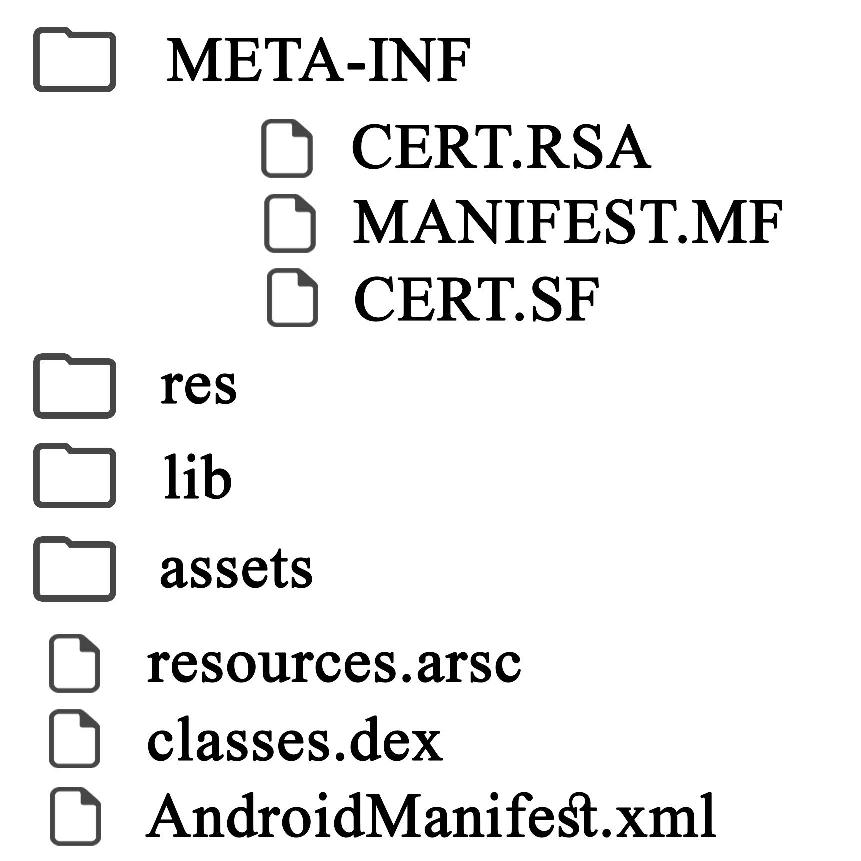
\includegraphics[width=60mm]{images/apkStructure.pdf}
  \end{center}
  \caption{Typická štruktúra APK súboru}
\end{figure}

\section{Priečinok META-INF}
\label{META-INF}
Priečinok obsahujúci súbory, ktorých úlohou je zaručiť integritu ostatných súborov v APK balíčku a s ňou spojenú bezpečnosť celého systému. V prípade detekcie pozmenených súborov a narušenia integrity operačný systém Android nedovolí inštaláciu APK balíčku. Po každej zmene je nutné balíček digitálne podpísať.


\subsection*{CERT.RSA}
\label{CERT.RSA} 
Súbor obsahujúci verejný kľúč ktorý slúži na overenie digitálneho podpisu balíčka.
\subsection*{MANIFEST.MF}
\label{MANIFEST.MF}
Súbor obsahujúci relatívne cesty a SHA-1 hashe \footnote{reťazce v Base64 kódovaní} všetkých súborov v APK balíčku. Tento súbor neobsahujú len APK súbory, je typický pre každý JAR archív.\\\\
Typický začiatok súboru \zv{MANIFEST.MF} vyzerá nasledovne: \\

\begin{verbatim}
Manifest-Version: 1.0
Built-By: 0.12.2
Created-By: Android Gradle 0.12.2

Name: res/drawable-xhdpi-v4/libraries.png
SHA1-Digest: VvgaO1jpW3iS1nBBikD/urdbN58=

Name: res/layout/activity_settings.xml
SHA1-Digest: 1coP1lt9Lmccc7SMZGHxNv4bbKs=
\end{verbatim}

\subsection*{CERT.SF}
\label{CERT.SF}
Súbor podobný ako \zv{MANIFEST.MF}, avšak namiesto SHA-1 hashov samotných súborov obsahuje SHA-1 hashe záznamov o týchto súboroch z \zv{MANIFEST.MF}. Okrem toho obsahuje aj hash celého súboru \zv{MANIFEST.MF}. \newline Záznam o jednom súbore v APK balíčku v súbore \zv{CERT.SF} vyzerá nasledovne: \newline
\begin{verbatim}
Name: res/drawable-xhdpi-v4/libraries.png
SHA1-Digest: Slg56lqothjvmaBikD/urdb7q6=
\end{verbatim}\mbox{}\\
Reťazec \zv{Slg56lqothjvmaBikD/urdb7q6=} reprezentuje SHA-1 hash nasledujúceho záznamu zo súboru \zv{MANIFEST.MF}:\mbox{}\\
\begin{verbatim}
“Name: res/drawable-xhdpi-v4/libraries.png
SHA1-Digest: VvgaO1jpW3iS1nBBikD/urdbN58=
”\end{verbatim}

\section{Priečinok res}
\label{res}
Priečinok obsahujúci zdrojové súbory ako napríklad obrázky, zvuky alebo ikony. Okrem multimediálnych súborov obsahuje taktiež zdrojové XML súbory určujúce vzhľad obrazoviek, použité grafické štýly, alebo texty použité v aplikácii. Niektoré z týchto XML súborov môžu byť skompilované do binárneho formátu. V zdrojovom kóde sú tieto zdroje odkazované pomocou unikátnych identifikátorov. Identifikátory sú generované počas kompilácie nástrojom aapt a nachádzajú sa v projektovej triede \zv{R}. Pre každý typ zdrojového súboru je generovaná podtrieda triedy \zv{R}. Všetky zdroje aplikácie by mali byť externalizované a uložené v špecifickom podpriečinku v tomto adresári. \\\\
\textbf{Podporované podpriečinky}
\begin{itemize}
\item animator - obsahuje XML súbory definujúce property animácie\cite{article-full}
\item anim - obsahuje XML súbory definujúce tween animácie, môže obsahovať aj property animácie
\item color - obsahuje XML súbory definujúce farby a ich zmeny na základe stavu objektov na ktoré sú aplikované
\item drawable - obsahuje obrázky vo formáte PNG, 9.PNG, JPG, GIF alebo XML súbory skompilované do formy vykresliteľných obrázkov
\item mipmap - ikony aplikácie s rôznou hustotou pixelov
\item layout - obsahuje súbory vo formáte XML definujúce vzhľad rozmiestnenie prvkov na obrazovke
\item menu - obsahuje súbory XML definujúce menu aplikácie
\item raw - obsahuje súbory ktoré musia byť uložené a použité v neskomprimovanej forme a kvalite
\item values - obsahuje súbory vo formáte XML definujúce hodnoty textových reťazcov, farieb, štýlov, základných rozmerov
\item xml - obsahuje XML súbory, ktoré môžu byť načítané počas behu aplikácie
\end{itemize}

\noindent V spomenutých priečinkoch sú uložené základné zdroje aplikácie. Tieto zdrojové súbory určujú základný dizajn a obsah aplikácie. Avšak rôzne typy Android zariadení môžu využívať rôzne zdrojové súbory. Alternatívne zdroje sa využívajú na prispôsobenie dizajnu a obsahu veľkosti a aktuálnej konfigurácií zariadenia. Sú umiestnené v priečinku, ktorého názov pozostáva z typu zdrojového súboru, ktorý korešponduje so základným názvom priečinku a názvu hodnoty konfiguračného atribútu pre ktorý je tento priečinok určený. Je možné kombinovať viacero konfiguračných atribútov.\\\\
\textbf{Najpoužívanejšie atribúty}
\begin{itemize}
\item Jazyk a región – jazyk je definovaný podľa ISO 639-1\footnote{http://www.iso.org/iso/home/standards/language\_codes.htm} kódovania s možnosťou rozšírenia pomocou ISO 3166-1-alpha-2 regionálneho kódu. Napríklad obrázky špecifické pre zariadenia s francúzskym jazykom sa nachádzajú v priečinku \cesta{res/drawable-fr}
\item Veľkosť obrazovky –  v závislosti na veľkosti a rozlíšení obrazovky rozlišuje štyri možné hodnoty -- small, normal, large, xlarge
\item Orientácia obrazovky – v závislosti na orientácii zariadenia hodnota port pre zariadenie vo vertikálnej polohe, hodnota land pre polohu horizontálnu
\item Hustota obrázkových bodov obrazovky -  hodnoty určujúce vhodnosť zdrojových súborov vzhľadom na hustotu obrázkových bodov obrazovky daného zariadenia
\end{itemize}


\section{Priečinok lib}
\label{lib}
Priečinok obsahujúci skompilovaný zdrojový kód natívnych knižníc. Tieto knižnice sú špecifické pre typ procesora. V závislosti na architektúre procesora obsahuje podpriečinky : \zv{armeabi, armeabi-v7a, arm64-v8a, x86, x86\_64, mips}.

\section{Priečinok assets}
\label{assets}
Priečinok obsahujúci súbory uložené a používané v originálnej neskomprimovanej forme. V tomto priečinku sa často nachádzajú textové súbory, html súbory, licenčné informácie, obrázky alebo textúry. Na rozdiel od priečinku \cesta{res/raw/}, zdrojovým súborom v umiestneným v priečinku assets nie sú pridelené unikátne identifikátory uložené v triede \zv{R.java}. K súborom sa pristupuje ako k dátam uloženým v bežnom súborovom systéme. Trieda \zv{AssetManager} poskytuje funkcionalitu na čítanie súborov ako prúdu bytov a  navigovanie v tomto priečinku.

\section{resources.arsc}
\label{resources.arsc}
Súbor obsahujúci mapovanie medzi zdrojovými súbormi  z priečinku \zv{res} a ich identifikátormi.  Vytvára sa počas kompilácie. Obsahuje XML súbory v binárnom formáte.

\section{classes.dex}
\label{classes.dex}
\zv{Classes.dex} je súbor obsahujúci skompilovaný zdrojový kód aplikácie.  Zdrojové súbory Android aplikácií sú napísané v jazyku Java. Java súbory sú skompilované do Java bytekódu pomocou bežného kompilátoru pre platformu Java. Výsledkom tejto kompilácie sú súbory s príponou \zv{class}, ktoré sú následne preložené do Dalvik bytekódu pomocou nástroja \zv{dx} ktorý je súčasťou Android Software Developement Kit. Výstupom nástroju \zv{dx} je jediný súbor obsahujúci skompilovaný celý výkonný zdrojový kód aplikácie -- \zv{classes.dex}. Tento súbor je skomprimovanou a optimalizovanou verziou všetkých \zv{class} súborov. Takto skompilovaný program môže byť vykonaný len vo virtuálnom stroji Dalvik, alebo v novšom prostredí ART (Android Runtime) používanom primárne od verzie Android 5.0 „Lollipop“.

\section{AndroidManifest.xml} 
\label{AndroidManifest.xml}
http://developer.android.com/guide/topics/manifest/manifest-intro.html
Súbor ktorý musí obsahovať každá Android aplikácia. Tento súbor poskytuje informácie o aplikácii operačnému systému Android. Neobsahuje žiadny výkonný kód. Definuje meno a verziu, ktoré slúžia ako unikátny identifikátor danej aplikácie. Popisuje všetky komponenty z ktorých sa aplikácia skladá, cesty k použitým knižniciam, minimálny vyžadovaný level Android API, oprávnenie vyžadované aplikáciu na prístup k chráneným častiam Android API a taktiež oprávnenia, ktoré sú vyžadované od iných komponent pri pokuse komunikovať s danou aplikáciou. Súbor \zv{AndroidManifest.xml}, ktorý nájdeme v APK balíčku je vo formáte binárneho XML súboru. Je ho však možné previesť do klasického čitateľného XML formátu.

Keďže \zv{AndroidManifest.xml} je základným súborom poskytujúcim metadáta o Android aplikácii a APK súbore, informácie získané z tohto súboru tvoria veľkú časť štatistických dát zbieraných a vyhodnocovaných v tejto práci. Preto sa detailnejšie pozrieme na jeho štruktúru a niektoré dôležité elementy, ktoré obsahuje.\\ Nasledujúci diagram ukazuje základnú štruktúru tohto XML súboru.
\begin{lstlisting} [language=XML, caption= {Základná štruktúra súboru AndroidManifest.xml}]
<?xml version="1.0" encoding="utf-8"?>
<manifest>
    <uses-permission />
    <permission />
    <uses-sdk />
    <uses-configuration />  
    <uses-feature />  
    <supports-screens />  
    <compatible-screens />  
    <application>
        <activity />
        <service/>
        <receiver/>
        <provider/>
        <uses-library />
    </application>
</manifest>
\end{lstlisting}

\subsection{Element manifest}
\lstset{language=XML}
\begin{lstlisting}
<manifest xmlns:android="URL"
          package="string"
          android:sharedUserId="string"
          android:sharedUserLabel="string resource"
          android:versionCode="integer"
          android:versionName="string"
          android:installLocation=["auto" | "internalOnly" |
                                        "preferExternal"] >
</manifest>
\end{lstlisting}
\zv{AndroidManifest.xml} obsahuje element manifest ako koreňový prvok. Tento element je povinný a každý manifest ho obsahuje práve jeden. \newline\newline
\noindent Element manifest definuje atribúty:\\
\begin{itemize}
\item xmlns:android – povinný atribút definujúci menný priestor
\item package – meno balíku aplikácie, povinný atribút definujúci identitu aplikácie. Meno balúku nemôže byť zmenené
\item android:sharedUserId – identifikátor aplikácie zdieľaný s ostatnými aplikáciami za účelom vzájomnej komunikácie
\item android:sharedUserLabel – čitateľná podoba android:sharedUserId identifikátoru
\item android:versionCode – interná informácia o verzii aplikácie. Tento atribút je využívaný len na rozoznanie novších verzíí od starších. Novšie aplikácie obsahujú vyššiu hodnotu
\item android:versionName – informácia o verzií aplikácie prezentovaná užívateľom. Pre systém Android neposkytuje informáciu o verzií aplikácie, tú obsahuje atribút android:versionCode.
\item android:installLocation – určuje miesto základné miesto inštalácie aplikácie. Pokiaľ je aplikáciu možné nainštalovať len do vnútornej pamäti zariadenia, obsahuje hodnotu internalOnly. Takáto aplikácia nemôže byť presunutá na externé pamäťové médium (typicky SD karta). Táto hodnota je základnou použitou možnosťou, ak tento atribút nie je definovaný. V prípade hodnoty auto sú aplikácie inštalované vo vnútornej pamäti, ale môžu byť presunuté do pamäti externej. Hodnota preferExternal zabezpečí, že systém sa pokúsi o inštaláciu na externé pamäťové médium. V prípade neúspechu sa použije interná pamäť
\end{itemize}

\subsection{Element uses-permission}
\lstset{language=XML}
\begin{lstlisting}
<uses-permission android:name="string"
        android:maxSdkVersion="integer" />
\end{lstlisting}
Prístup k niektorým dátam alebo častiam kódu je z dôvodu ochrany limitovaný. Android využíva princíp povolení\footnote{angl. permissions}. Povolenia môžu byť definované samotnou aplikáciou, inou aplikáciou alebo systémom Android. Aplikácia, ktorá chce pristupovať k chráneným dátam alebo používať chránené časti kódu, musí pomocou tagu uses-permissions deklarovať vyžadované povolenia. Prístupové povolenia sú aplikácii schválené užívateľom. Vo verzii Android 5.1 a starších, systém počas inštalácie oboznámi užívateľa so všetkými povoleniami, ktoré aplikácia vyžaduje. V prípade, že ich používateľ neschváli, aplikácia nebude nainštalovaná. Od verzie Android 6.0 užívateľ schvaľuje povolenia počas behu aplikácie.\\\\ 
Element uses-permission definuje atribúty:\\
\begin{itemize}
\item android:name – definuje názov povolenia
\item android:maxSdkVersion – najvyšší level Android API, pre ktorý je dané povolenie potrebné
\end{itemize}

\subsection{Element permission}
\lstset{language=XML}
\begin{lstlisting}
<permission android:description="string resource"
            android:icon="drawable resource"
            android:label="string resource"
            android:name="string"
            android:permissionGroup="string"
            android:protectionLevel=["normal"|"dangerous"| 
                                     "signature"|
                                     "signatureOrSystem"] />
\end{lstlisting}
Definuje bezpečnostné povolenie, ktoré môže byť použité na obmedzenie prístupu ku komponente aplikácie. Toto povolenie je následne používané aplikáciami, ktoré vyžadujú prístup k chránenej časti danej aplikácie.\\\\ Najdôležitejšie atribúty definované v rámci elementu permission:\\
\begin{itemize}
\item android:name – názov povolenia, aplikácie vyžadujúce dané povolenie uvádzajú túto hodnotu v atribúte android:name v tagu uses-permission. Názov musí byť unikátny a mal by dodržiavať konvencie pomenovávania jazyka Java.
\item android:permissionGroup – priradí toto povolenie do skupiny povolení (angl. Permission group). Táto skupina povolení musí byť deklarovaná v rámci elementu permission-group v niektorej z nainštalovaných aplikácií. Slúži na logické zoskupenie významovo podobných oprávnení.
\item android:protectionLevel – charakterizuje potenciálne riziko spojené s použitím daného povolenia. Táto hodnota určuje postup operačného systému pri rozhodovaní o udelení povolenia. 
Základnou hodnotou je „normal“, ktorá reprezentuje povolenia s nízkou mierou rizika. Tieto povolenia sú aplikácii automaticky schválené systémom Android počas inštalácie. Pre povolenia z zvýšenou mierou rizika je určená hodnota „dangerous“. Tieto povolenia typicky udeľujú aplikácií prístup k citlivým dátam alebo k prvkom Android zariadenia, ktoré môžu negatívne ovplyvniť jeho používanie. Pretože tento typ povolení prináša potenciálne riziko, systém ho nemôže udeliť automaticky, ale až po explicitnom súhlase používateľa.
V prípade, že tento atribút obsahuje hodnotu „signature“, povolenie je udelené automaticky a to len aplikáciám, ktorých certifikát je rovnaký ako certifikát aplikácie definujúcej dané povolenie.   
Hodnota „signatureOrSystem“ rozširuje hodnotu „signature“ a povolenia sú udelené aj aplikáciám Android system image.
\end{itemize}

\subsection{Element uses-sdk}
\lstset{language=XML}
\begin{lstlisting}
<uses-sdk android:minSdkVersion="integer"
          android:targetSdkVersion="integer"
          android:maxSdkVersion="integer" />
\end{lstlisting}
Element vyjadrujúci kompatibilitu aplikácie s verziou Androidu pomocou čísla verzie Android API.\\\\
Atribúty definované elementom uses-sdk:\\
\begin{itemize}
\item android:minSdkVersion – vyjadruje najnižší level API vyžadovaný aplikáciou. Pokiaľ je táto hodnota vyššia ako API úroveň zariadenia, systém zabráni inštalácií. Tento atribút by mala obsahovať každá aplikácia
\item android:targetSdkVersion – informuje o úrovni API na ktorej bola aplikácia testovaná a pre ktorú je primárne určená. V prípade, že zariadenie podporuje vyššiu verziu Android API ako definuje spomínaný atribút, aplikácia môže byť spustená v móde kompatibility s touto verziou API 
\item android:maxSdkVersion – najvyššia úroveň API kompatibilná s aplikáciou. Z dôvodu spätnej kompatibility nie je používanie tohto atribútu doporučené. Tento atribút bol využívaný len do verzie Android 2.0.1
\end{itemize}

\subsection{Element uses-feature}
\lstset{language=XML}
\begin{lstlisting}
<uses-feature
  android:name="string"
  android:required=["true" | "false"] />
\end{lstlisting}
Deklaruje hardvérovú alebo softvérovú vlastnosť \footnote{angl. feature} používanú aplikáciou. Tento element informuje externé entity o funkciách, ktoré aplikácia vyžaduje. Deklarované vlastnosti majú informačný charakter. Systém Android nekontroluje či zariadenie podporuje všetky vlastnosti deklarované aplikáciou. Tento element je využívaný službou Google Play na  filtrovanie aplikácií vyhovujúcich danému zariadeniu, a preto by mala byť deklarovaná každá vyžadovaná vlastnosť.\\\\ Element obsahuje nasledujúce atribúty:\\
\begin{itemize}
\item android:name – názov vyžadovanej vlastnosti
\item android:required – určuje, či aplikácia vyžaduje danú vlastnosť pre korektné fungovanie. Pokiaľ obsahuje hodnotu true, aplikácia nie je schopná korektne fungovať na zariadení nepodporujúcom danú vlastnosť
\end{itemize}

http://developer.android.com/guide/topics/manifest/uses-feature-element.html
\subsection{Element supports-screens}
\lstset{language=XML}
\begin{lstlisting}
<supports-screens android:resizeable=["true"| "false"]
                  android:smallScreens=["true" | "false"]
                  android:normalScreens=["true" | "false"]
                  android:largeScreens=["true" | "false"]
                  android:xlargeScreens=["true" | "false"]
                  android:anyDensity=["true" | "false"]
                  android:requiresSmallestWidthDp="integer"
                  android:compatibleWidthLimitDp="integer"
                  android:largestWidthLimitDp="integer"/>
\end{lstlisting}
Špecifikuje podporované typy obrazoviek. V prípade inštalácie na zariadení s väčšou obrazovkou ako aplikácia podporuje, informuje systém o potrebe využitia módu obrazovej kompatibility.\\\\ Väčšina atribútov deklaruje podporované veľkosti obrazoviek. Ďalšie atribúty využívané v tejto práci sú:\\
\begin{itemize}
\item android-resizeable – indikuje schopnosť aplikácie korektne sa prispôsobiť rôznym veľkostiam obrazoviek
\item android:anyDensity – indikuje či aplikácia obsahuje zdrojové súbory vhodné pre obrazovky s rôznou hustotu obrazových bodov
\end{itemize}

\subsection{Element activity}
Deklaruje aktivity. Aktivity sú základnými časťami aplikácie. Sú to triedy rozširujúce triedu \zv{android.app.Activity}. Sú zamerané na jednotlivé prípady použitia aplikácie, implementujú časť grafické užívateľského rozhrania a zabezpečujú komunikáciu s užívateľom. Tieto triedy sú časťou zdrojového kódu a v skompilovanej forme sa nachádzajú v súbore classes.dex. Pri viacerých spustených aktivitách zohráva dôležitú úlohu životný cyklus aktivity. Viac informácií o životnom cykle aktivít nájdete na (http://developer.android.com/reference/android/app/Activity.html). Všetky aktivity musia byť deklarované pomocou tagu activity. V prípade, že deklarované nie sú, systém ich bude ignorovať a nebudú spustené. Syntax a kompletný zoznam atribútov definovaných v tagu activity môžete nájsť na http://developer.android.com/guide/topics/manifest/activity-element.html. 

\subsection{Element service}
Deklaruje komponenty aplikácie typu služba\footnote{angl. service}. Na rozdiel od aktivít, služby nemajú grafické používateľské rozhranie. Slúžia na implementáciu dlhodobých úloh na pozadí, ktoré môžu bežať aj v čase keď aplikácia nie je aktívna na popredí, alebo poskytujú funkcionalitu využívanú aplikáciou. Rozlišujeme dva typy služieb. Služby typu started po spustení bežia pokým nedokončia svoju úlohu a ostatným komponentom nevracajú výsledok. Služby typu bound komunikujú s ostatnými komponentami pomocou modelu klient-server a sú ukončené keď pre nich neexistuje klient.  Každá služba rozširuje základnú triedu \zv{android.app.Service} a musí byť deklarovaná pomocou elementu service, inak bude ignorovaná. Syntax prvku service môžete nájsť na http://developer.android.com/guide/topics/manifest/service-element.html
\subsection{Element provider}
Deklaruje komponenty aplikácie ktorých úlohou je poskytovanie štrukturovaného prístupu k dátam spravovaným aplikáciou. Poskytovatelia obsahu \footnote{angl. content providers} sú implementovaný ako podtriedy triedy \zv{ android.content.ContentProvider}. Využitie tejto komponenty je nutné len v prípade potreby zdieľania dát medzi viacerými aplikáciami. Operačný systém Android si ukladá referencie na jednotlivých poskytovateľov obsahu pomocou authority textového reťazca, ktorý je definovaný ako jeden z atribútov elementu provider. Kompletný list atribútov sa nachádza na http://developer.android.com/guide/topics/manifest/provider-element.html. Systém Android si nerozpoznáva poskytovateľov obsahu nedefinovaných v AndroidManifest.xml.
\subsection{Element receiver}
Deklaruje komponentu aplikácie implementovanú ako podtriedu triedy \zv{android.content.BroadcastReceiver}. Tieto komponenty umožňujú aplikácií prijímať a reagovať na informácie o zámere spustenia aktivity (intent) aj v čase, keď ostatné komponenty aplikácie nie sú spustené. Tieto informácie sú vysielané systémom alebo inou aplikáciou. Systém Android môžeme oboznámiť s existenciou komponent typu broadcast receiver pomocou tagu receiver alebo aj dynamicky pomocou volania \zv{Context.registerReceiver()} v zdrojovom kóde aplikácie. Kompletný list atribútov sa nachádza na http://developer.android.com/guide/topics/manifest/receiver-element.html
\subsection{Element uses-library}
\lstset{language=XML}
\begin{lstlisting}
<uses-library
  android:name="string"
  android:required=["true" | "false"] />
\end{lstlisting}
Špecifikuje zdieľanú knižnicu vyžadovanú aplikáciou. Tento element informuje systém o potrebe zahrnúť cestu k zdrojovému kódu knižnice medzi cesty v ktorých Dalvik Virtual Machine hľadá zdrojové súbory. V angličtine sú tieto cesty označované ako class path. Najpoužívanejšie android balíky ako napríklad android.app, android.content alebo android.view sú obsiahnuté v základnej knižnici, ktorá je automaticky pripojená ku každej aplikácií a nemusia byť deklarované týmto elementom. Balíčky, ktoré nie sú v základnej android knižnici, musia byť deklarované.  Tento element ovplyvňuje inštaláciu aplikácie na konkrétnom zariadení a taktiež dostupnosť aplikácie v obchode Google Play.\\\\ Definuje atribúty:\\
\begin{itemize}
\item android:name – názov knižnice, ktorý sa nachádza v dokumentácií príslušného použitého balíčku
\item android:required – indikuje či aplikácia potrebuje knižnicu špecifikovanú atribútom android:name. V prípade hodnoty true aplikácia nie je schopná fungovať bez danej knižnice. Systém zamietne inštaláciu takejto aplikácie, pokiaľ zariadenie neobsahuje danú knižnicu. 	Ak je tento atribút nastavený na hodnotu false, aplikácia je schopná korektne fungovať aj bez danej knižnice
\end{itemize}



%% Apk databáza
\chapter{Databáza inštalačných APK súborov}
Základnou úlohou tejto práce je vytvoriť dostatočne veľkú databázu inštalačných APK balíčkov. Pre ďalšie potreby práce je požadované, aby veľká časť aplikácií pochádzala z~neoficiálnych zdrojov, čím sa zvyšuje pravdepodobnosť, že aplikácia bola modifikovaná alebo obsahuje malvér.

Naša databáza pozostáva približne z~20000 Android aplikácií. Tie boli zaobstarané v~časovom rozmedzí medzi novembrom 2015 a februárom 2016. Žiadna z~aplikácií nebola stiahnutá priamo z~obchodu \zv{Google Play}. Oficiálny zdroj \zv{Google Play Store} neumožňuje priame sťahovanie APK súborov. Žiadosť na stiahnutie APK súboru musí byť asociovaná s~Google účtom a konkrétnym Android zariadením prepojeným s~daným účtom pomocou jednoznačného identifikátoru \zv{ANDROID-ID}. Open source projekt \zv{Google Play Crawler}~\cite{gpCrawler} založený na neoficiálnom \zv{Google Play API}~\cite{gpApi} umožňuje limitovaný prístup, prehľadávanie a aj sťahovanie aplikácií z~\zv{Google Play Store}. Získavanie APK súborov pomocou \zv{Google Play Crawler} nebolo možné efektívne realizovať kvôli zastaralosti a funkčným obmedzeniam neoficálneho \zv{Google Play API}, ktoré bolo naposledy upravené v~roku 2012.

Veľká časť APK súborov bola získaná s~využitím projektu \zv{Playdrone}. V~rámci tohto projektu bolo v~novembri 2014 z~\zv{Google Play} stiahnutých viac ako milión aplikácií dostupných pre zariadenie \zv{Galaxy Nexus} s~operátorom \zv{T-Mobile}~\cite{Viennot2014}. Naša databáza obsahuje 8200 najsťahovanejších aplikácií z~\zv{Google Play} v~období november 2014, ktoré boli stiahnuté z~archívu projektu \zv{Playdrone}. Ostatné aplikácie boli prevzaté z~neoficiálnych webových lokalít určených na distribúciu aplikácií, ale aj pomocou torrent súborov, alebo zo stránok na zdielanie ľubovoľného obsahu.

Celková veľkosť všetkých stiahnutých APK súborov je 192\,GB. Prehľad všetkých zdrojov APK súborov a ich počet zobrazuje tabuľka \ref{tab:stahovanie}. 

\begin{table}[htb]
\centering
  \begin{tabular}{|l r r|}
    \hline
    \textbf{Zdroj} & \textbf{Počet aplikácií} & \textbf{\%} \\\hline\hline
    Playdrone & 8200 & 40,9\\
    www.appsapk.com & 6470 & 32,3\\
    www.apkmaniafull.com & 2870 & 14,3\\
    www.androidapksfree.com & 1030 & 5,1\\
    www.zippyshare.com & 750 & 3,7\\
    torrenty & 550 & 2,7\\
    www.uloz.to & 190 & 0,9\\
    \midrule\hline
    Spolu & 20060 & \\
    \hline
  \end{tabular}
  \caption{Zdroje prevzatých APK súborov}
  \label{tab:stahovanie}
\end{table}


\section{Implementácia}
Viac ako 90\,\% aplikácií bolo stiahnutých automatizovane prostredníctvom aplikácie \zv{ApkDownloader} implementovanej v~rámci tejto práce. Aplikácia neposkytuje grafické užívateľské rozhranie, ale užívateľ môže zadávať parametre prostredníctvom príkazového riadku. \zv{ApkDownloader} funguje na jednoduchom princípe, keď najskôr získa zoznam URL odkazov na APK súbory, ktoré následne stiahne. Podporuje sťahovanie aplikácií získaných pomocou projektu \zv{Playdrone} alebo z~nasledujúcich neoficiálnych lokalít zameraným na distribúciu Android aplikácií: 
\begin{itemize}
 \item \zv{www.appsapk.com},
 \item \zv{www.apkmaniafull.com},
 \item \zv{www.androidapksfree.com}.
\end{itemize}

V~prípade sťahovania aplikácií z~archívu projektu \zv{Playdrone}~\cite{Viennot2014} je potrebné špecifikovať súbor s~metainformáciami obsahujúci odkazy na APK súbory. Tento súbor sa nachádza v~archíve projektu \zv{Playdrone}~\cite{archiveOrg}. Žiadny zo spomínaných zdrojov neposkytuje verejné API na prístup a sťahovanie súborov. Pri ostatných podporovaných zdrojoch \zv{ApkDownlaoder} vyhľadá odkazy na APK súbory v~HTML kóde príslušnej stránky. Vyhľadávanie odkazov je priamo závislé na HTML kóde danej webovej stránky a jeho zmena môže mať vplyv na korektné fungovanie aplikácie. Keďže je \zv{ApkDownloader} open source, môže byť jednoducho adaptovaný na zmenený HTML kód, ale aj rozšírený o~podporu sťahovania APK súborov z~nových lokalít. Za účelom rozšíriteľnosti a jednoduchej modifikovateľnosti poskytuje \zv{ApkDownlaoder} jednoduché verejné API. Použitie \zv{ApkDownlaoder} je zobrazené v~ukážke kódu 4.1, ktorá reprezentuje telo metódy \zv{main} danej aplikácie. \\
\begin{lstlisting} [language=java, basicstyle=\small\color{black},frame=single,framesep=10pt, caption= {\zv{ApkDownloader} API a jeho použitie} \label{downlaoderCode}]
ApkLinkFinder finder = arguments.getLinkFinder();
finder.setMetadataFile(arguments.getMetadataFile());
finder.setNumberOfApks(arguments.getNumberOfApks());
List<String> urls = finder.findLinks();

ApkDownloader downloader = arguments.getApkDownloader();
downloader.setDownloadDirectory(arguments.getDownloadDirectory());
downloader.setNumberOfThreads(arguments.getNumberOfThreads());
downloader.setOverwriteExisting(arguments.isOverwriteExisting());
downloader.download(urls);
\end{lstlisting}
\mbox{}\\
\noindent Užívateľ pomocou parametrov špecifikuje z~ktorej podporovanej lokality chce APK súbory stiahnuť, ich želaný počet, umiestnenie prebraných súborov a maximálny počet súbežných preberaní. Pri vyhľadávaní URL odkazov je na prácu s~HTML súbormi použitá open source knižnica \zv{jsoup}. Pri sťahovaní sa využíva knižnica \zv{HtmlUnit}, ktorá poskytuje funkcionalitu internetového prehliadača. Na preberanie súborov z~URL odkazov je použitá knižnica \zv{Apache Commons IO}. 

Torrent súbory boli získane automatizovane s~využitím knižnice \zv{flux}~\cite{flux}. \zv{Flux} poskytuje API na vyhľadávanie a sťahovanie torrent súborov z~portálu \zv{www.torrentz.eu}. Tento nástroj je implementovaný v~prostredí NodeJS. Samotné APK súbory boli následne prevzaté prostredníctvom bežného torrent klienta.

\chapter{These are}
\section{the available}
\subsection{sectioning commands.}
\paragraph{Paragraphs and}
\subparagraph{subparagraphs are available as well.}
Inside the text, you can also use unnumbered lists,
\begin{itemize}
  \item such as
  \item this one
  \begin{itemize}
    \item     and they can be nested as well.
    \item[>>] You can even turn the bullets into something fancier,
    \item[\S] if you so desire.
  \end{itemize}
\end{itemize}
Numbered lists are
\begin{enumerate}
  \item very
  \begin{enumerate}
    \item similar
  \end{enumerate}
\end{enumerate}
and so are description lists:
\begin{description}
  \item[Description list]
    A list of terms with a description of each term
\end{description}
The spacing of these lists is geared towards paragraphs of text.
For lists of words and phrases, the \textsf{paralist} package
offers commands
\begin{compactitem}
  \item that
  \begin{compactitem}
    \item are
    \begin{compactitem}
      \item better
      \begin{compactitem}
        \item suited
      \end{compactitem}
    \end{compactitem}
  \end{compactitem}
\end{compactitem}
\begin{compactenum}
  \item to
  \begin{compactenum}
    \item this
    \begin{compactenum}
      \item kind of
      \begin{compactenum}
        \item content.
      \end{compactenum}
    \end{compactenum}
  \end{compactenum}
\end{compactenum}


\chapter{Floats and references}
\begin{figure}
  \begin{center}
    %% PNG and JPG images can be inserted into the document as well,
    %% but their resolution needs to be adequate. The minimum is
    %% about 250 pixels per 1 centimeter. That means that a JPG or
    %% PNG image typeset at 40 × 40 mm should be 1000 × 1000 px
    %% large at minimum.
    \includegraphics[width=40mm]{fithesis/logo/mu/fithesis-base.pdf}
  \end{center}
  \caption{The logo of the Masaryk University at 40\,mm}
  \label{fig:mulogo1}
\end{figure}

\begin{figure}
  \begin{minipage}{.66\textwidth}
    \includegraphics[width=\textwidth]{fithesis/logo/mu/fithesis-base.pdf}
  \end{minipage}
  \begin{minipage}{.33\textwidth}
    \includegraphics[width=\textwidth]{fithesis/logo/mu/fithesis-base.pdf} \\
    \includegraphics[width=\textwidth]{fithesis/logo/mu/fithesis-base.pdf}
  \end{minipage}
  \caption{The logo of the Masaryk University at $\frac23$ and
    $\frac13$ of text width}
  \label{fig:mulogo2}
\end{figure}

\begin{table}
  \begin{tabularx}{\textwidth}{lllX}
    \toprule
    Day & Min Temp & Max Temp & Summary \\
    \midrule
    Monday & $13^{\circ}\mathrm{C}$ & $21^\circ\mathrm{C}$ & A
    clear day with low wind and no adverse current advisories. \\
    Tuesday & $11^{\circ}\mathrm{C}$ & $17^\circ\mathrm{C}$ & A
    trough of low pressure will come from the northwest. \\
    Wednesday & $10^{\circ}\mathrm{C}$ &
    $21^\circ\mathrm{C}$ & Rain will spread to all parts during the
    morning. \\
    \bottomrule
  \end{tabularx}
  \caption{A weather forecast}
  \label{tab:weather}
\end{table}

The logo of the Masaryk University is shown in Figure
\ref{fig:mulogo1} and Figure \ref{fig:mulogo2} at pages
\pageref{fig:mulogo1} and \pageref{fig:mulogo2}. The weather
forecast is shown in Table \ref{tab:weather} at page
\pageref{tab:weather}. The following chapter is Chapter
\ref{chap:matheq} and starts at page \pageref{chap:matheq}.
Items \ref{item:star1}, \ref{item:star2}, and
\ref{item:star3} are starred in the following list:
\begin{compactenum}
  \item some text
  \item some other text
  \item $\star$ \label{item:star1}
  \begin{compactenum}
    \item some text
    \item $\star$ \label{item:star2}
    \item some other text
    \begin{compactenum}
      \item some text
      \item some other text
      \item yet another piece of text
      \item $\star$ \label{item:star3}
    \end{compactenum}
    \item yet another piece of text
  \end{compactenum}
  \item yet another piece of text
\end{compactenum}
If your reference points to a place that has not yet been typeset,
the \verb"\ref" command will expand to \textbf{??} during the first
run of
\texttt{pdflatex \jobname.tex}
and a second run is going to be needed for the references to
resolve. With online services -- such as Overleaf -- this is
performed automatically.

\chapter{Mathematical equations}
\label{chap:matheq}
\TeX{} comes pre-packed with the ability to typeset inline
equations, such as $\mathrm{e}^{ix}=\cos x+i\sin x$, and display
equations, such as \[
  \mathbf{A}^{-1} = \begin{bmatrix}
  a & b \\ c & d \\
  \end{bmatrix}^{-1} =
  \frac{1}{\det(\mathbf{A})} \begin{bmatrix}
  \,\,\,d & \!\!-b \\ -c & \,a \\
  \end{bmatrix} =
  \frac{1}{ad - bc} \begin{bmatrix}
  \,\,\,d & \!\!-b \\ -c & \,a \\
  \end{bmatrix}.
\] \LaTeX{} defines the automatically numbered \texttt{equation}
environment:
\begin{equation}
  \gamma Px = PAx = PAP^{-1}Px.
\end{equation}
The package \textsf{amsmath} provides several additional
environments that can be used to typeset complex equations:
\begin{enumerate}
  \item An equation can be spread over multiple lines using the
    \texttt{multline} environment:
    \begin{multline}
      a + b + c + d + e + f + b + c + d + e + f + b + c + d + e +
f \\
      + f + g + h + i + j + k + l + m + n + o + p + q
    \end{multline}

  \item Several aligned equations can be typeset using the
    \texttt{align} environment:
    \begin{align}
              a + b &= c + d     \\
                  u &= v + w + x \\[1ex]
      i + j + k + l &= m
    \end{align}

  \item The \texttt{alignat} environment is similar to
    \texttt{align}, but it doesn't insert horizontal spaces between
    the individual columns:
    \begin{alignat}{2}
      a + b + c &+ d       &   &= 0 \\
              e &+ f + g   &   &= 5
    \end{alignat}

  \item Much like chapter, sections, tables, figures, or list
    items, equations -- such as \eqref{eq:first} and
    \eqref{eq:mine} -- can also be labeled and referenced:
    \begin{alignat}{4}
      b_{11}x_1 &+ b_{12}x_2  &  &+ b_{13}x_3  &  &             &
        &= y_1,                   \label{eq:first} \\
      b_{21}x_1 &+ b_{22}x_2  &  &             &  &+ b_{24}x_4  &
        &= y_2. \tag{My equation} \label{eq:mine}
    \end{alignat}

  \item The \texttt{gather} environment makes it possible to
    typeset several equations without any alignment:
    \begin{gather}
      \psi = \psi\psi, \\
      \eta = \eta\eta\eta\eta\eta\eta, \\
      \theta = \theta.
    \end{gather}

  \item Several cases can be typeset using the \texttt{cases}
    environment:
    \begin{equation}
      |y| = \begin{cases}
        \phantom-y & \text{if }z\geq0, \\
                -y & \text{otherwise}.
      \end{cases}
    \end{equation}
\end{enumerate}
For the complete list of environments and commands, consult the
\textsf{amsmath} package manual\footnote{
  See \url{http://mirrors.ctan.org/macros/latex/required/amslatex/math/amsldoc.pdf}.
  The \texttt{\textbackslash url} command is provided by the
  package \textsf{url}.
}.

\chapter{\textnormal{We \textsf{have} \texttt{several} \textsc{fonts}
  \textit{at} \textbf{disposal}}}
The serified roman font is used for the main body of the text.
\textit{Italics are typically used to denote emphasis or
quotations.} \texttt{The teletype font is typically used for source
code listings.} The \textbf{bold}, \textsc{small-caps} and
\textsf{sans-serif} variants of the base roman font can be used to
denote specific types of information.

\tiny We \scriptsize can \footnotesize also \small change \normalsize
the \large font \Large size, \LARGE although \huge it \Huge
is \huge usually \LARGE not \Large necessary.\normalsize

A wide variety of mathematical fonts is also available, such as: \[
  \mathrm{ABC}, \mathcal{ABC}, \mathbf{ABC}, \mathsf{ABC},
  \mathit{ABC}, \mathtt{ABC}
\] By loading the \textsf{amsfonts} packages, several additional
fonts will become available: \[
  \mathfrak{ABC}, \mathbb{ABC}
\] Many other mathematical fonts are available\footnote{
  See \url{http://tex.stackexchange.com/a/58124/70941}.
}.

\chapter{Inserting the bibliography}
After loading the \texttt{biblatex} package and linking a
bibliography data\-base file to the document using the
\verb"\addbibresource" command, you can start citing the entries.
This is just dummy text \cite{inbook-full} lightly sprinkled with
citations \cite[p.~123]{incollection-full}.  Several sources can be
cited at once \cite{whole-collection, manual-minimal,manual-full}.
\citetitle{inbook-full} was written by \citeauthor{inbook-full} in
\citeyear{inbook-full}. We can also produce \textcite{inbook-full}
or%% Let us define a compound command:
\def\citeauthoryear#1{(\textcite{#1},~\citeyear{#1})}
\citeauthoryear{inbook-full}. The full bibliographic citation is:
\emph{\fullcite{inbook-full}}. We can easily insert a bibliographic
citation into the footnote\footfullcite{inbook-full}.

The \verb"\nocite" command will not generate any
output\nocite{booklet-full}, but it will insert its argument into
the bibliography. The \verb"\nocite{*}" command will insert all the
records in the bibliography database file into the bibliography.
Try uncommenting the command
\nocite{*}
and watch the bibliography section come apart at the seams.

When typesetting the document for the first time, citing a
\texttt{work} will expand to [\textbf{work}] and the
\verb"\printbibliography" command will produce no output. It is now
necessary to generate the bibliography by running \texttt{biber
\jobname.bcf} from the command line and then by typesetting the
document again twice. During the first run, the bibliography
section and the citations will be typeset, and in the second run,
the bibliography section will appear in the table of contents.

The \texttt{biber} command needs to be executed from within the
directory, where the \LaTeX\ source file is located. In Windows,
the command line can be opened in a directory by holding down the
\keys{Shift} key and by clicking the right mouse button while
hovering the cursor over a directory.  Select the \menu{Open
Command Window Here} option in the context menu that opens shortly
afterwards.

With online services -- such as Overleaf -- all commands are
executed automatically.

{\csname captions\languagename\endcsname %% Temporarily override
%% the BibLaTeX localization with the original babel definitions.
\makeatletter %% Use the correct localization of the quotations.
  \thesis@selectLocale{\thesis@locale}\makeatother
\printbibliography[heading=bibintoc]} %% Print the bibliography.
\begin{thebibliography}{9}
\bibitem{Westenberg2015}
WESTENBERG, Jimmy. Gartner: Android and iOS dominate smartphone market with 98 percent marketshare. \textit{Android Authority} [online]. 2015 [cit. 2016-03-20]. Dostupné z: http://www.androidauthority.com/android-ios-hold-98-percent-marketshare-656624/

\end{thebibliography}
\chapter{Inserting the index}
After using the \verb"\makeindex" macro and loading the
\texttt{makeidx} package that provides additional indexing
commands, index entries can be created by issuing the \verb"\index"
command. \index{dummy text|(}It is possible to create ranged index
entries, which will encompass a span of text.\index{dummy text|)}
To insert complex typographic material -- such as $\alpha$
\index{alpha@$\alpha$} or \TeX{} \index{TeX@\TeX} --
into the index, you need to specify a text string, which will
determine how the entry will be sorted. It is also possible to
create hierarchal entries. \index{vehicles!trucks}
\index{vehicles!speed cars}

After typesetting the document, it is necessary to generate the
index by running
\begin{center}%
  \texttt{texindy -I latex -C utf8 -L }$\langle$\textit{locale}%
  $\rangle$\texttt{ \jobname.idx}
\end{center}
from the command line, where $\langle$\textit{locale}$\rangle$
corresponds to the main locale of your thesis -- such as
\texttt{english}, and then typesetting the document again.

The \texttt{texindy} command needs to be executed from within the
directory, where the \LaTeX\ source file is located. In Windows,
the command line can be opened in a directory by holding down the
\keys{Shift} key and by clicking the right mouse button while
hovering the cursor over a directory. Select the \menu{Open Command
Window Here} option in the context menu that opens shortly
afterwards.

With online services -- such as Overleaf -- the commands are
executed automatically, although the locale may be erroneously
detected, or the \texttt{makeindex} tool (which is only able to
sort entries that contain digits and letters of the English
alphabet) may be used instead of \texttt{texindy}. In either case,
the index will be ill-sorted.

%\makeatletter\thesis@blocks@clear\makeatother
\phantomsection %% Print the index and insert it into the
\addcontentsline{toc}{chapter}{\indexname} %% table of contents.
\printindex

\appendix %% Start the appendices.
\chapter{An appendix}
Here you can insert the appendices of your thesis.

\end{document}
